\chapter{Evaluation}
In this chapter, we evaluate our system on the basis of reliability, scalability, and network longevity.

\section{Reliability}\label{sec:reliability}

\begin{figure}[htbp]
\centering
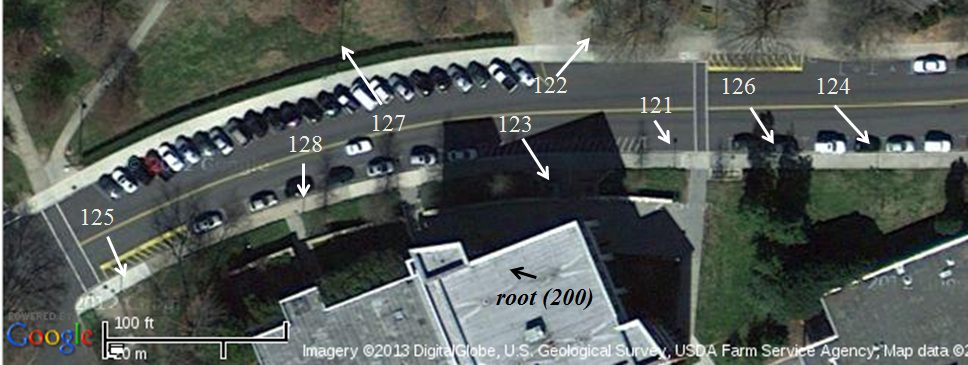
\includegraphics[width=\columnwidth]{img_deployment.png}
\caption{Mote Deployment}
\label{img_deployment}
\end{figure}

\begin{figure}[htbp]
\centering
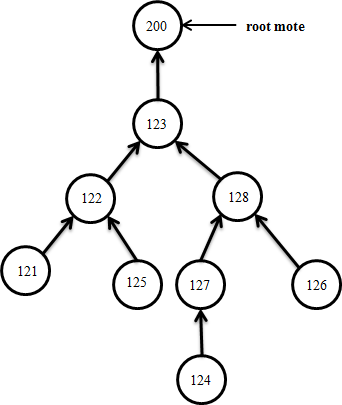
\includegraphics[width=8cm]{network.png}
\caption{Observed Routing Topology}
\label{img_network}
\end{figure}

In this section, we evaluate the reliability of the network based on two parameters: the percentage error in packet reception, and the ability of the network to tolerate mote failure.
%, and the ability to eliminate partition of network.
 To evaluate these parameters we deployed eight motes on the lamp posts in front of Clemson University's School of Computing. The \textit{\textbf{root}} mote was deployed inside the School of Computing, as shown in Figure \ref{img_deployment}. The \textit{\textbf{root}} mote was connected to a desktop server process and periodically received data from the deployed motes. Figure \ref{img_network} shows the observed routing topology formed by the deployed motes.

\subsection{Percentage Error in Packet Reception}\label{sec:percentage_error}
In this subsection, we evaluate the percentage error in packet reception for each mote in the network. The percentage error in packet reception is defined as the ratio of the difference between the number of packets transmitted by the mote and the number of packets received at the base station, to the number of packets transmitted. That is, we consider end-to-end packet reception. To evaluate the percentage error in packet reception, we allowed the deployed motes to run continuously for 7 days. Each data packet sent by a mote to its parent contained a count of the total number of tries it took to successfully send the message, as well as the message number of the data being transferred. Table \ref{table_dataTransmitted} shows the total number of packets transmitted, the total number of packets received, the percentage error in packet reception, and the total number of tries before successful transmission of the packets over a period of 7 days.
%To evaluate the yield of the network we deployed eight motes on the light polls in front of School of Computing, Clemson University, and the \textit{\textbf{root}} mote is deployed inside School of Computing. The \textit{\textbf{root}} mote is connected to the field deployed server and periodically receives data from the deployed motes. The deployed motes are (some (suggestion)) meters apart.
%The data packet sent by the motes contains the number of tries by the mote before the parent mote received that packet and the count of message it transferred to the parent mote. We also calculate the error in packet reception for each mote. We maintain the count of packets received from each mote at the base station.


\begin{table}[htbp]
\begin{center}
\begin{tabular}{|c|c|c|c|c|}
\hline 
\textbf{Mote} & \textbf{Count of} & \textbf{Count of} & \textbf{Percentage error} & \textbf{Total number} \\ 
 &   \textbf{packets}   &  \textbf{packets}  & \textbf{in packet} & \textbf{of retries}\\
 & \textbf{transmitted}  & \textbf{received} & \textbf{reception} & \\
\hline  
\hline  
121 & 8714 & 8714 & 0 & 122 \\ 
\hline 
122 & 9047 & 9047 & 0 & 344 \\  
\hline 
123 & 10152 & 10152 & 0 & 4 \\ 
\hline 
124 & 8129 & 8129 & 0 & 161 \\ 
\hline 
125 & 9282 & 9282 & 0 & 165 \\ 
\hline 
126 & 6240 & 6240 & 0 & 184 \\  
\hline 
127 & 9182 & 9182 & 0 & 64 \\ 
\hline 
128 & 5195 & 5195 & 0 & 389 \\ 
\hline 
\hline
\textbf{Total} & 65941 & 65941 & 0 & 1433 \\
\hline
\end{tabular}
\end{center}
\caption{Data Transmission Metrics}
\label{table_dataTransmitted}
\end{table}

As we can see from Table \ref{table_dataTransmitted}, the percentage error in packet reception is 0. The packets transmitted by each mote are received at the base station. That is, the network achieved 100\% data yield. The number of retries before successful transmission of a data packet is less than 3\% of the total packets transmitted by all motes.

%To check the reliability of the network when there are lots of packets in network we ran the same test as above with one extra mote in the network which constantly broadcast a packet of data every 10 milli second to make the network congested, during that scenario the error rate is less than one percent.

\subsection{Ability to Tolerate Mote Failure}\label{sec:tolerate_mote_failure}
In this subsection, we evaluate the ability of the network to withstand mote failures. To evaluate this property of the network, we followed the same experimental setup described in sections \ref{sec:reliability} and \ref{sec:percentage_error}. Figure \ref{img_network} shows the observed routing topology formed by the deployed motes. To evaluate the ability of the network to withstand mote failure, we introduced a fault by deactivating mote 128. Due to this, motes 127, 126, and 124 were disconnected from the network. We observed that motes 127, 126, and 124 detected the failure of mote 128, and rejoined the network, choosing another parent.
% We can see from Tables \ref{table_selfHealingSystem} and \ref{table_selfHealingMote}, all of the failed motes rejoined the network.

Regular (i.e., real) failure cases were also considered. Here, failure is defined as the removal of the mote from the network due to an obstruction between motes, an out of range mote, power failure, or a mote in the process of resetting. To determine the failure of the mote, we monitor the data received at the base station and timestamp the data. If the data is not received from a particular mote for 5 minutes then the mote is declared as failed. After that, whenever data is received from the failed mote, we conclude that the mote rejoined the network. Table \ref{table_selfHealingSystem} shows, over a period of a day, the number of mote failures recorded,  the number of rejoins that occurred within 10 minutes, and the number of failures that persisted beyond 10 minutes. Table \ref{table_selfHealingMote} shows, for each mote, over a period of 7 days, the number of failures the mote experienced, the number of times the mote was able to rejoin the network after a failure, and the number of times the mote was unable to rejoin the network after a failure. These figures suggest that the network is able to withstand mote failure.
% To evaluate the self-healing property of the network we deployed eight motes on the light polls in front of School of Computing, Clemson University, and the \textit{\textbf{root}} mote is deployed inside School of Computing. The \textit{\textbf{root}} mote is connected to the field deployed server and periodically receives data from the deployed motes. The deployed motes are (some (suggestion)) meters apart.To evaluate the self-healing property of the network, we kept the deployed motes running continuously for 7 days. The data packet sent by the motes contains the number of tries by the mote before the parent mote received that packet and the count of message it transferred to the parent mote. Table \ref{table_selfHealingSystem} shows the number of motes failed, number of motes recovered, and number of motes unable to recover within 10 minutes each day on the system level. Table \ref{table_selfHealingMote} shows the number of failures, number of recoveries, and number of times unable to recover for each mote over a period of 7 days.

\begin{table}[htbp]
\begin{center}
\begin{tabular}{|c|c|c|c|}
\hline 
\textbf{Day} & \textbf{Number of mote} & \textbf{Number of failures} & \textbf{Failures not} \\ 
 & \textbf{failures} & \textbf{corrected within} & \textbf{corrected within} \\ 
 &   & \textbf{10 minutes}  & \textbf{10 minutes} \\
\hline 
\hline 
June 20 & 4 & 4 & 0 \\ 
\hline 
June 21 & 48 & 48 & 0 \\ 
\hline 
June 22 & 56 & 55 & 1 \\ 
\hline 
June 23 & 42 & 40 & 2 \\ 
\hline 
June 24 & 61 & 61 & 0 \\ 
\hline 
June 26 & 29 & 29 & 0 \\ 
\hline 
June 27 & 18 & 18 & 0 \\ 
\hline 
\end{tabular}
\end{center} 
\caption{Mote Failure Statistics (per day)}
\label{table_selfHealingSystem}
\end{table}


\begin{table}[htbp]
\begin{center}
\begin{tabular}{|c|c|c|c|}
\hline 
\textbf{Mote} & \textbf{Number of} & \textbf{Number of failures} & \textbf{Failures not} \\ 
 & \textbf{failures} & \textbf{corrected within} & \textbf{corrected within} \\ 
 &   & \textbf{10 minutes}  & \textbf{10 minutes} \\
\hline 
\hline 
121 & 7 & 7 & 0 \\ 
\hline 
122 & 9 & 9 & 0 \\ 
\hline 
123 & 0 & 0 & 0 \\ 
\hline 
124 & 9 & 9 & 0 \\ 
\hline 
125 & 9 & 9 & 0 \\ 
\hline 
126 & 38 & 38 & 0 \\ 
\hline 
127 & 5 & 5 & 0 \\ 
\hline 
128 & 181 & 178 & 3 \\ 
\hline 
\end{tabular}
\end{center} 
\caption{Mote Failure Statistics (per mote)}
\label{table_selfHealingMote}
\end{table}

Table \ref{table_selfHealingSystem} shows that one mote was unable to recover on June 22, and two motes were unable to recover on June 23. We can see from Table \ref{table_selfHealingMote} that the only mote that was unable to recover is mote 128. The failure of mote 128 was purposefully introduced by disconnecting the battery. We can see from Tables \ref{table_selfHealingSystem} and \ref{table_selfHealingMote} that every other mote eventually recovered and rejoined the network within 10 minutes after failing. This supports our claims that the network is able to withstand mote failures.

%\subsection{Partition-free Network} 
%If a mote fails it divides the network in two subsets. In this subsection we evaluate our system and show that it is partition-free i.e. it prevents the network from partitioning. To evaluate the partition-free property of the network, we allowed the deployed motes to run continuously for 7 days. Each data packet, sent by a mote to its parent, contains a count of the total number of tries it took to successfully send the message, as well as the message number being transferred. Table \ref{table_partitionFreeSystem} shows the number of motes failed, number of motes recovered, and number of motes unable to recover each day.

%To evaluate the partition property of the network, we kept the deployed motes running continuously for 7 days. The data packet sent by the motes contains the number of tries by the mote before the parent mote received that packet and the count of message it transferred to the parent mote. Table \ref{table_partitionFreeSystem} shows the number of motes failed, number of motes recovered, and number of motes unable to recover each day.

%\begin{table}[htbp]
%\begin{center}
%\begin{tabular}{|c|c|c|c|}
%\hline 
%\textbf{Day} & \textbf{Number of motes} & \textbf{Number of motes} & \textbf{Number of motes} \\ 
% & \textbf{Failed} & \textbf{recovered} & \textbf{unable to recover} \\ 
%\hline 
%\hline 
%• & • & • & • \\ 
%\hline 
%• & • & • & • \\ 
%\hline 
%• & • & • & • \\ 
%\hline 
%• & • & • & • \\ 
%\hline 
%• & • & • & • \\ 
%\hline 
%• & • & • & • \\ 
%\hline 
%• & • & • & • \\ 
%\hline 
%• & • & • & • \\ 
%\hline 
%\end{tabular}
%\end{center} 
%\caption{Partition-free System}
%\label{table_partitionFreeSystem}
%\end{table}


%We can see from Table \ref{table_partitionFreeSystem} that every mote recovers after failing, and joins the original network, and does not form a new network. This proves that the network is partition-free.

The results presented in sections \ref{sec:percentage_error} and \ref{sec:tolerate_mote_failure} support our claim that the network is reliable.

\section{Scalability}
This section evaluates the scalability of our system. In this context, scalability depends on the internal message buffer size, the number of transmission slots per mote, and the baud-rate of the transceiver.

Internal buffer size is an important factor in the evaluation of network scalability. In the experiments discussed in the previous sections, the size of the internal message buffer is 255 bytes, and the size of a data packet is 7 bytes. The maximum number of motes allowed in each transmission slot of the \textit{\textbf{root}} mote in the network is equal to the number of message packets that can be accommodated in the internal message buffer. It is assumed that each mote transmits exactly one data packet.
\begin{center}
$number\ of\ motes\ =\ \dfrac{255}{7}\ =\ 36.43$
\end{center}

Since the \textit{root} mote immediately transmits all received data to the base station, the network can accommodate 36 motes \textit{per child} of the \textit{root} mote, assuming an internal buffer size of 255 bytes per mote and a message packet size of 7 bytes.

The total number of motes that can be accommodated in a network, depends on the number of transmission slots per mote. In our system, the duration of each transmission slot is 3 seconds (calculated in Section \ref{sec:trans_slots}), and data is transmitted every 60 seconds. Therefore, the total number of transmission slots that can be present in each period is $\dfrac{60\ (second)}{3\ (second)}\ =\ 20\ slots$. The total number of motes that can be accommodated in our system is as follows:

\begin{equation}
T_{motes}\ = N_{slots}*N_{motes} 
\end{equation}


\begin{tabular}{lllp{10cm}}
where, &   &   &   \\ 
%\hline 
  & $T_{motes}$  & = & the maximum number of motes that can be accommodated in the network \\ 
%\hline 
  & $N_{slots}$ & = & the maximum number of transmission slots in a transmission period \\ 
%\hline 
  & $N_{motes}$ & = & the maximum number of motes in each transmission slot of the \textit{\textbf{root}} mote \\ 
\end{tabular} 
%where,\\
%$T_{motes}$ = the maximum number of motes that can be accommodated in the network\\
%$N_{slots}$ = the maximum number of transmission slots in a transmission period\\
%$N_{motes}$ = the maximum number of motes in each transmission slot of \textit{\textbf{root}} mote\\

\begin{center}
$T_{motes}\ =\ 20\ *\ 36\ =\ 720\ motes$.
\end{center}

The baud-rate of the transceiver is also an important factor in the scalability of the network. The baud-rate of the RFM12 transceiver is 57.6 Kbps. The number of bytes that can be transmitted in one transmission slot, i.e. 3 seconds, is as follows:
\begin{center}
$number\ of\ bytes\ =\ \dfrac{3*57600}{8}\ =\ 21600$
\end{center}

Now we calculate the maximum number of bytes that can be transmitted in 3 seconds. The equation is as follows: 

\begin{equation}
T_{max} = N_{motes}*D_{bytes}
\end{equation}

\begin{tabular}{lllp{10cm}}
where, &   &   &   \\ 
  & $T_{max}$  & = & the maximum number of bytes transmitted during each transmission \\ 
  & $N_{motes}$ & = & the maximum number of motes in each transmission slot of the \textit{\textbf{root}} mote \\ 
  & $D_{bytes}$ & = & the size of a data message, including packet overhead \\ 
\end{tabular} 

\begin{center}
$T_{max}\ =\ 36\ *\ 12\ =\ 432\ bytes$
\end{center}
In our system, even if each mote sends its data 20 times, we transmit a maximum of 8640 bytes (432 * 20) in 3 seconds per mote. The radio can easily handle the transmitted data.% The maximum data that can be transmitted by 720 motes in a period of 60 second is 288000 bytes.

The calculations for internal buffer size, number of transmission slots per mote, and baud-rate of the transceiver together show that given the buffer size of 255 bytes and a message packet size of 7 bytes, this network can scale to accommodate 720 motes. To increase the number of motes beyond 720, we must increase the internal message buffer size.


\section{Network Longevity}
This section evaluates the longevity of the network. Here, network longevity is defined as the time period for which the network will work. The circuit operates both in the absence and presence of sunlight. We consider the lifetime of network in both cases.

\subsection{Absence of Sunlight}\label{subsec:sunlight_absent}
This subsection considers the lifetime of the network running only on battery power, in the absence of sunlight. Table \ref{table_powerConsumption} shows the power consumption of the microcontroller and the RFM12 transceiver in the active and sleep states.
\begin{table}[htbp]
\begin{center}
\begin{tabular}{|c|c|c|c|}
\hline 
   & \textbf{Micro-} & \textbf{RFM12} & \textbf{Total} \\ 
  &  \textbf{controller} &  &   \\ 
\hline 
\hline 
\textbf{active} & 4.00 & 9.00 & 13.00 + $\alpha_{1}$ \\ 
\hline 
\textbf{sleep} & 0.52 & 0.10 & 0.62 + $\alpha_{2}$ \\ 
\hline 
\end{tabular}
\end{center} 
\caption{Device Current Consumption ($milliamps$)}
\label{table_powerConsumption}
\end{table}

Our system works at a 10\% duty cycle; the motes transmit data every 60 seconds. Within a 60 second timeframe, the motes are in the active state for 6 seconds, and in the sleep state for 54 seconds (assumed each mote has maximum 2 children). The current consumption is calculated using the following formula:
\begin{equation} \label{equ:current_consumption}
C = \frac{A*on\ time + S*off\ time}{total\ time}
\end{equation}
%where,\\
%C = Current consumption in $\ milliAmps$\\
%A = Active state power consumption\\
%S = Sleep state power consumption\\

\begin{tabular}{lllp{10cm}}
where, & • & • & • \\ 
• & C & = & Current consumption in $\ milliamps$ \\ 
• & A & = & Active state current consumption in $\ milliamps$ \\ 
• & S & = & Sleep state current consumption in $\ milliamps$ \\ 
\end{tabular} 

\begin{center}
$C = \dfrac{6*13.00 + 54*0.62}{60} = 1.858 \ milliamps$
\end{center}
The lifetime of a mote is calculated using the following formula:
\begin{equation}
Lifetime = \frac{Battery\ Capacity*0.80}{Current\ Consumption}
\end{equation}
The 0.80 in the equation indicates that we can use up to 80\% of the battery to run the circuit.
\begin{center}
$Lifetime\ =\ \dfrac{850*0.80}{1.858}\ =\ 365.98\ hrs\ =\ 15.25\ days$\\
\end{center}

The above calculation indicates that the network can run on battery power, in the absence of sunlight, for a period of 15.25 days.

\subsection{Presence of Sunlight}\label{subsec:sunlight_present}
This subsection evaluates the lifetime of the network running in the presence of sunlight. The solar panel generates 89 milliamps of current, and a voltage of 5 volts. Of the 89 milliamps of current, the solar panel supplies 17 milliamps of current to the processing circuit, and it supplies 50 milliamps of current to charge the Li-Ion battery. The remaining 12 milliamps of current is not used.

As calculated in equation \ref{equ:current_consumption}, the mote consumes 1.858 milliamps of current. Let us assume that sunlight is available for 6 hours each day. As stated above, the solar panel will charge the battery by 6 * 50 = 300 mAh (best case charging). Each day, circuit runs on the battery for 18 hours. The power consumption from the battery is 18 * 1.858 = 33.44 mAh. As we can see, energy consumed is just 11.148 \% of the energy stored each day.

The above calculations in subsections \ref{subsec:sunlight_absent} and \ref{subsec:sunlight_present} support our claim that the network will function properly for long periods without changing the batteries.
\newpage
%--------------------------------------------------------------------------------------


%To evaluate this hardware and software solution we created ten motes. The mote as shown in Figure %\ref{img_prototypeBoard} consists of solar power circuit, battery circuit, switching circuit, and processing circuit.

%To test that the network is forming correctly, is reliable, partition free, and scalable, we setup the experiment in \textit{Dependable Systems Research Group} lab, \textit{Clemson University}. We deployed seven motes in the lab at different locations. In this experiment the motes were connected to fixed power supply.

%To test the working of solar power circuit, we placed three motes outside in sunlight.

%We placed the mote with Root status in lab, this mote is connected to the base station. The base station records the data and the number of packets received. The id of the mote with status Root is 200 and the id of other motes ranges from 101 to 109.

%[Note: The networks are dynamically formed when this program is used, for simplicity all the images of the network below are of same type, means the location of motes are fixed in the images]

%\section{Network formation}

%\begin{figure}
%\centering
%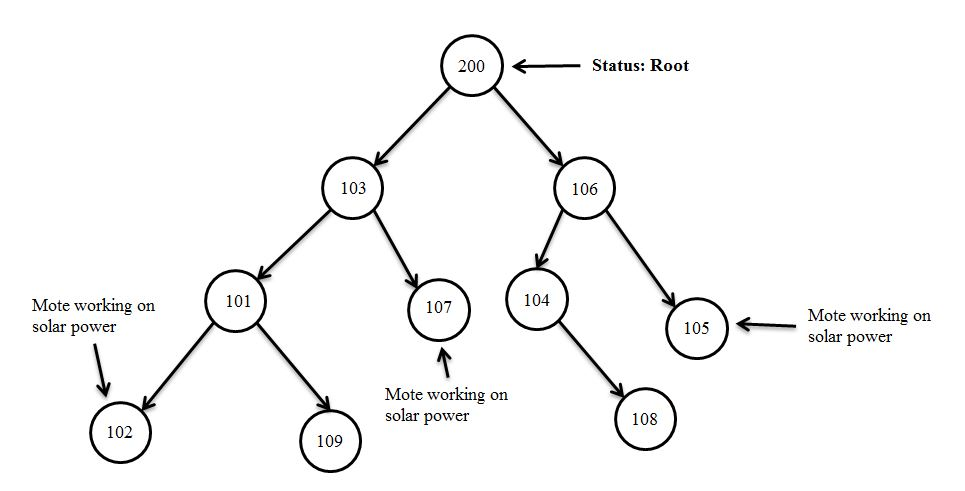
\includegraphics[width=\columnwidth]{network.JPG}
%\caption{Network formed}
%\label{img_network}
%\end{figure}

%In this experiment the mote with status of Root (id 200) is connected to the base station. The other motes when they wake up has status of idle. As discussed in section 3.2 they perform operations 1, 2, 3, 4, and 5 and forms the network. 
%The network formed by these motes is shown in Figure \ref{img_network}. All of the motes from id 101 to 109 tries to connect to the Root but only motes with id 103 and 106 succeeds in connecting with the mote id 200 in the first try. Now as mote with id 200 don't have any slots available, the other motes cannot join it. Whenever motes with id 103 and 106 get time synchronized with their parent the remaining motes can join them. This process is repeated until all the motes in idle state join the network.


%\section{Scalable}

%\begin{figure}
%\centering
%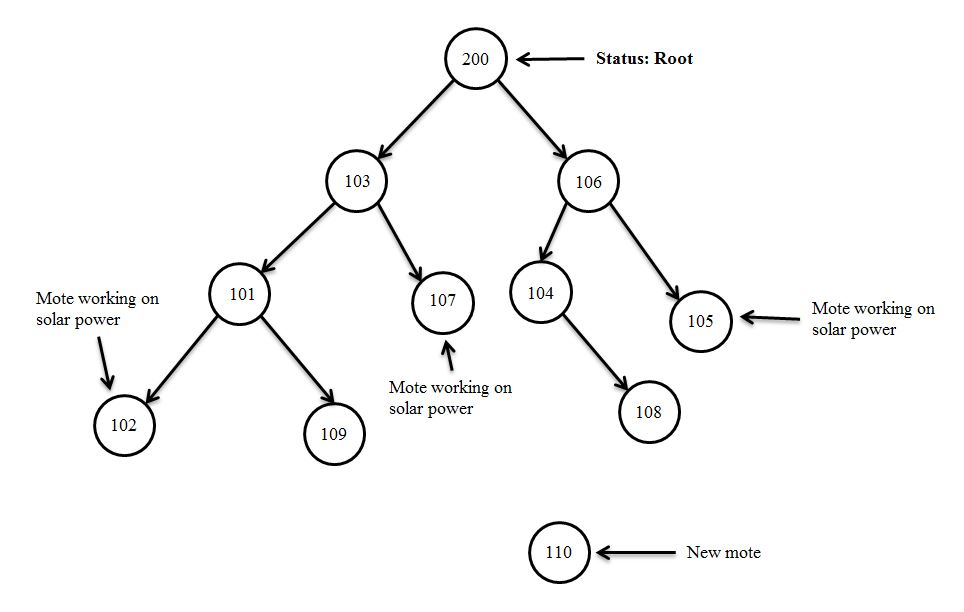
\includegraphics[width=\columnwidth]{network1.JPG}
%\caption{Scalable network}
%\label{img_network1}
%\end{figure}
%As shown in Figure \ref{img_network1}, if new mote (mote id 110 as indicated in Figure \ref{img_network1}) wants to join the  network. It performs operation 1 as discussed in section 3.2, If there is mote awake at that time and has free time slot available then operations 2, 3, 4, and 5 takes place and the new mote joins the network.

%To check the scalability function of the network, instead of waking all the motes at the same time, we wake up one mote at a time. We added nine motes using this technique and all the motes joined the network. This shows that the network formed using this software is scalable.


%\section{Partition free}

%\begin{figure}
%\centering
%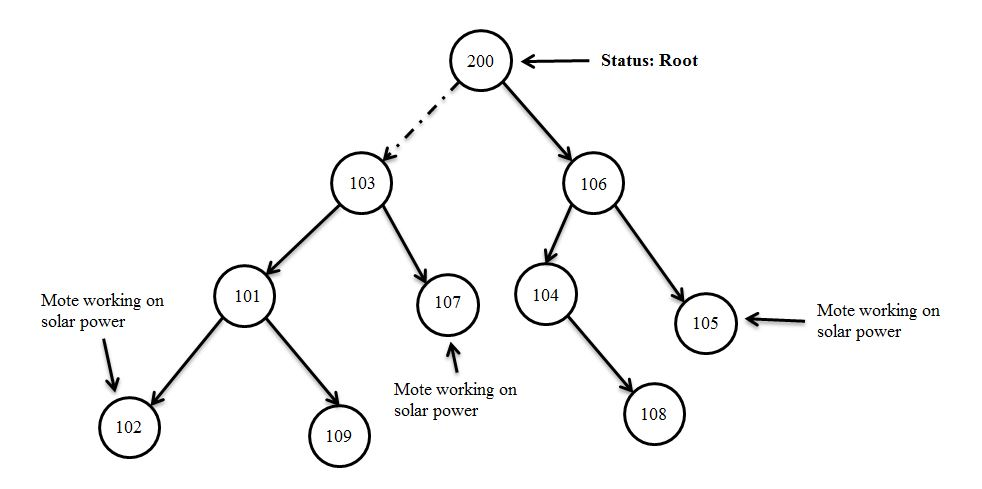
\includegraphics[width=\columnwidth]{network2.JPG}
%\caption{Partition free network}
%\label{img_network2}
%\end{figure}

%To evaluate that the network cannot remain partitioned for a longer period of time, as shown in Figure \ref{img_network2} we deliberately broke the link between mote id 200 and mote id 103 by changing the address of the parent of the mote id 103. This caused the network to break in two parts, one part consisting of mote id 200 as the Root mote and other part consisting of mote id 103 as the root mote. As a result of this scenario  mote id 103 stopped receiving synchronization signal. As the status of mote id 103 is Node it recognized this situation as the death of its parent. After detecting the death of the parent, mote id 103 propagated this death to is child and killed itself. All the motes connected to mote 103 killed themselves on reciving this signal as a result of operation 8 as discussed in section 3.2 . In the next step they again joined the network as new motes. This solved the problem of partition in the network.

%\section{Self healing}To evaluate the self healing property of the network, we intentionally killed mote 103, the already formed network is as shown in Figure \ref{img_network}. As a result of this motes 101 and 107 stopped receiving the synchronization signal, because of this they detected the death of their parent. Motes 101 and 107 then propagated the death to their child. After this the motes killed themselves. As discussed in section 3.2 Operation 8 takes place on the child motes and they also propagate the death to their child and killed themselves.